\section{Model Architectures}
\subsection{Baseline model: Fully Convolutional Network \tpdf{\phantom{xx}\small\texttt{models/SimpleFCN.py}}}

\begin{figure}[h]
    \centering 
    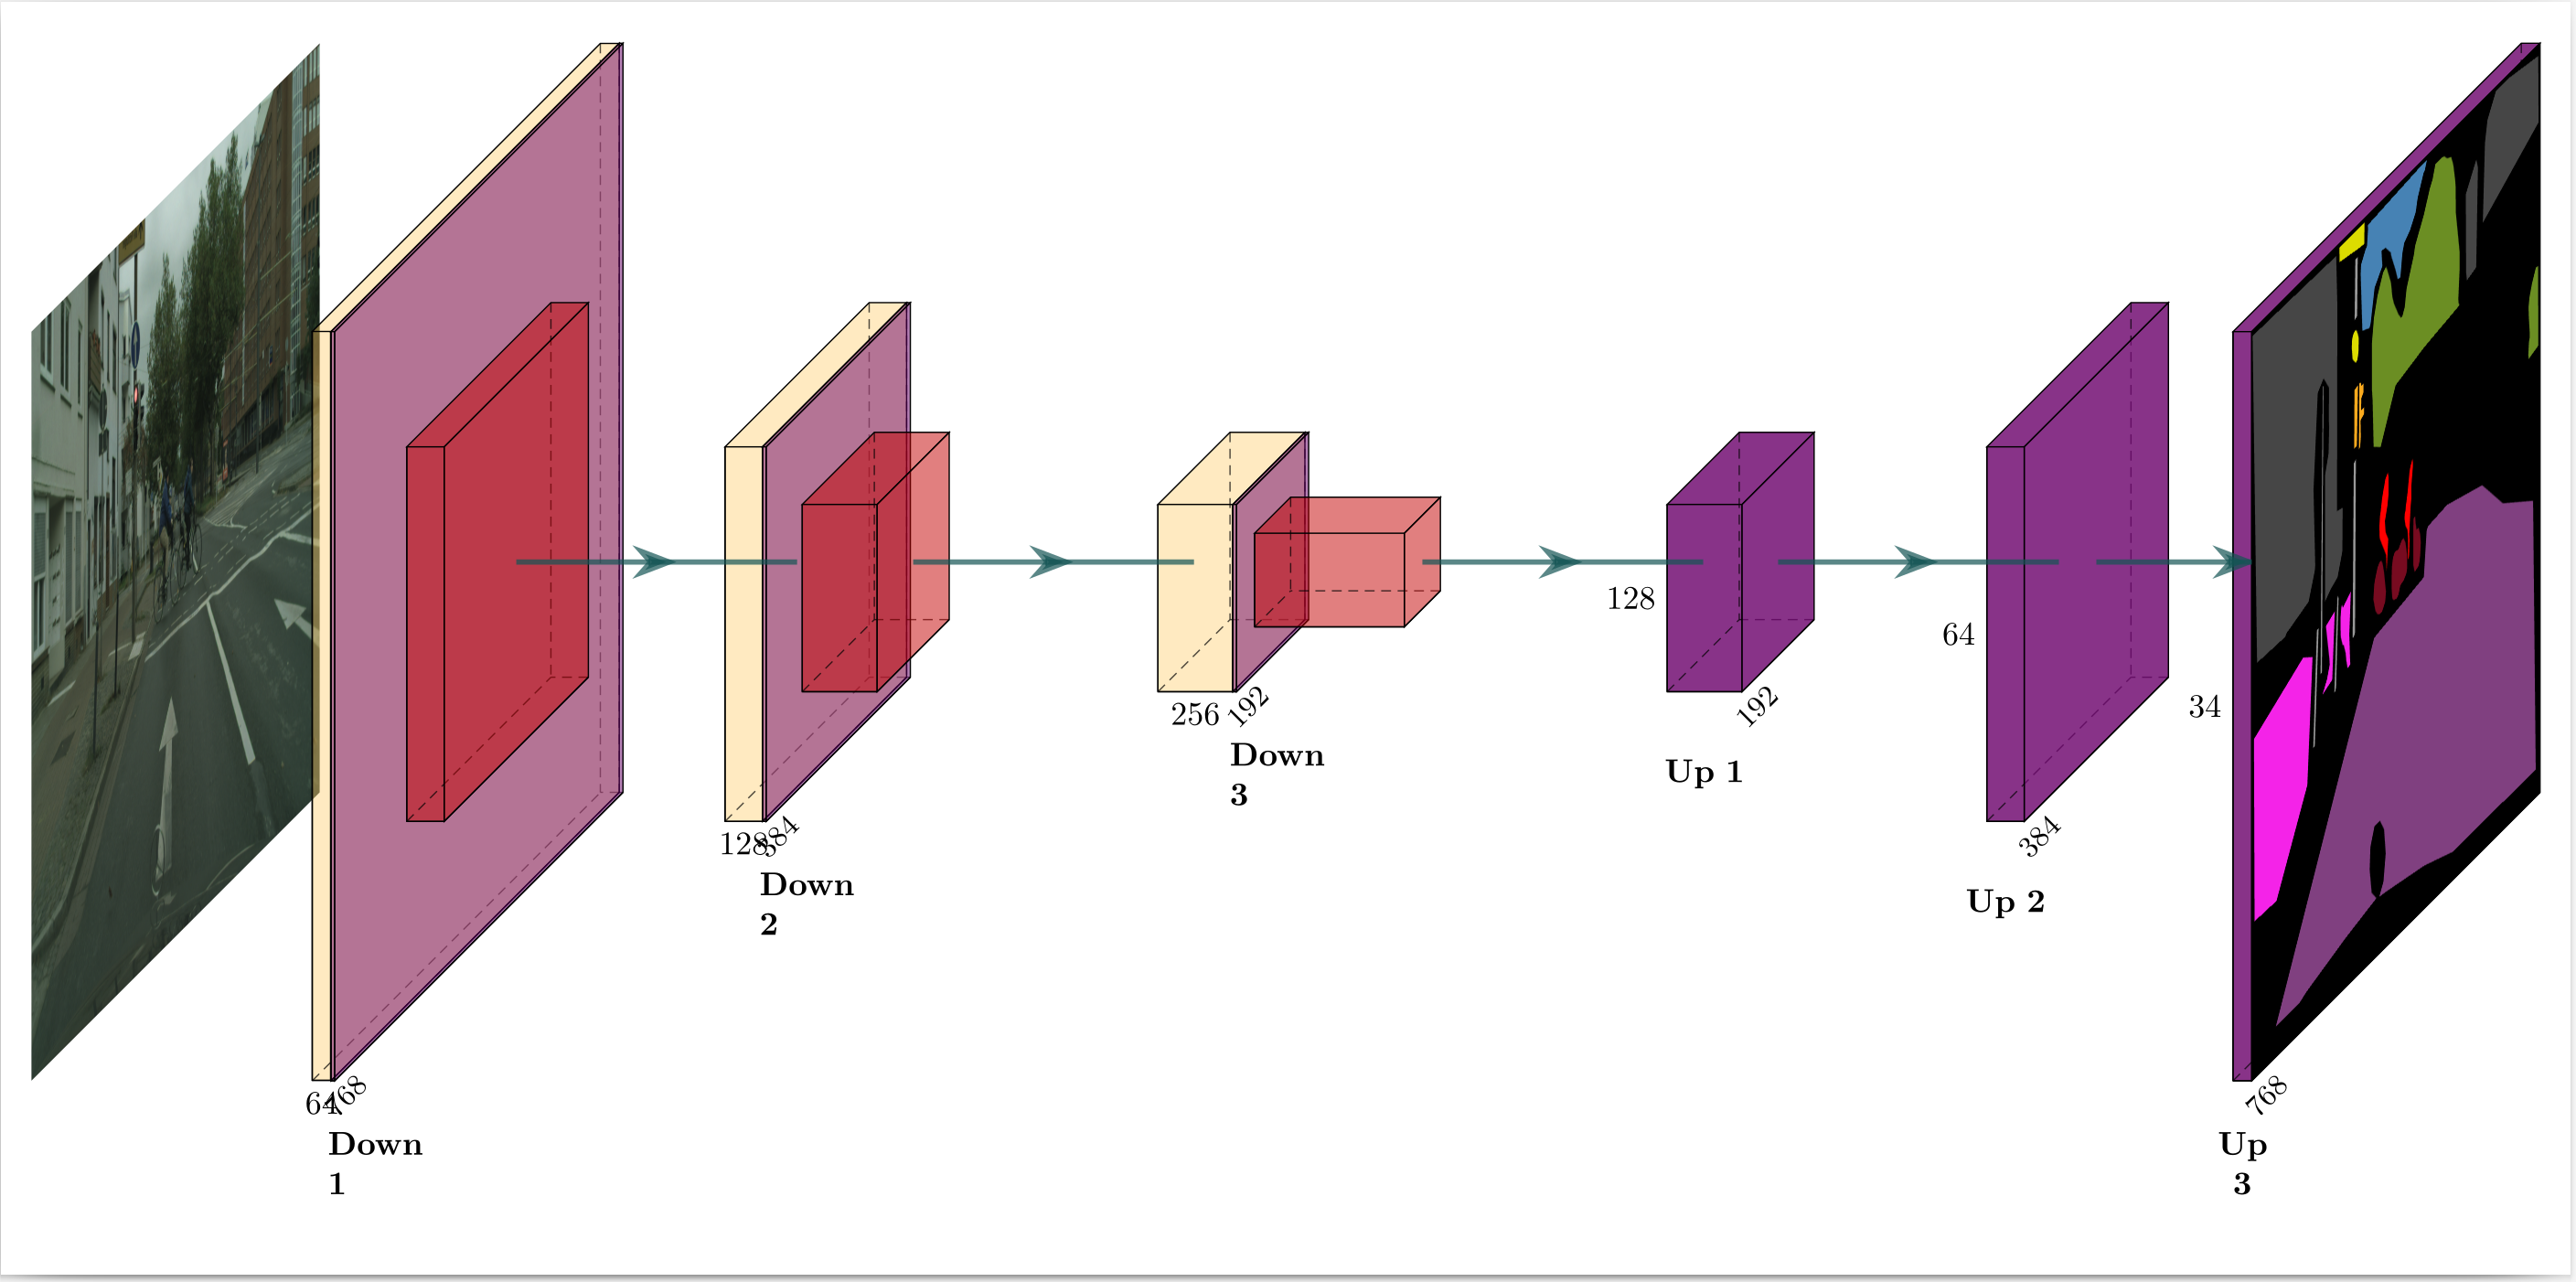
\includegraphics[width=0.6\textwidth]{SimpleFCN.png}
    \caption{The architecture of the baseline model}
    \label{baseline_model}
\end{figure}

Modern, state-of-the-art techniques for image analysis involve convolutional neural networks (CNNs) in their implementation. CNNs can be used to extract vital information from spatial features, which allow us to classify and segment objects in images. A type of neural network architecture designed specifically for semantic segmentation is the Fully Convolutional Network (FCN). This architecture, developed by researchers from UC Berkeley in 2014 \cite{DBLP:journals/corr/LongSD14}, has been influential in advancing the field of computer vision, particularly in tasks requiring dense prediction, like semantic segmentation. 

Our baseline model, illustrated in \cref{baseline_model}, is a simple fully-convolutional network with 3 encoding and 3 decoding steps. Images and masks have been resized to a square shape of 768$\times$768 pixels when loading the dataset. This allowed us to have increased efficiency in terms of computational resources, while not sacrificing too much performance. 

\begin{description}
	\item[Each encoding step] \phantom{hello}
		\begin{enumerate}
			\item Conv2D layer with kernel size $3 \times 3$ and simple padding to double of channels.
			\item ReLU layer to add some non-linearity.
			\item Max-pooling layer with kernel size $2 \times 2$ to ensure the following encoding layer gathers less local data.
		\end{enumerate}
	\item[Each decoder step] \phantom{hello}
		\begin{enumerate}
			\item Transposed convolution with kernel size $2 \times 2$, which halves the amount of channels and doubles the size of the image.
		\end{enumerate}
\end{description}

This model produces a result that's \textit{good enough}, but it can be improved by adding a bit of complexity.

Following are two enhanced models, both with a significantly better result.

\newpage{}
\subsection{Enhanced Model 1: UNet \tpdf{\phantom{MMMMMMMMMMMMx}\small\texttt{models/UNet.py}}}

The first enhanced model for our image segmentation task is a UNet model\cite{unet}.

This produces an encoder-decoder architecture that's not too dissimilar to our baseline model, but it has the addition of skip connections so that the transposed convolutions get data with different resolution as seen in \cref{unet}.

\begin{figure}[h]
    \centering 
    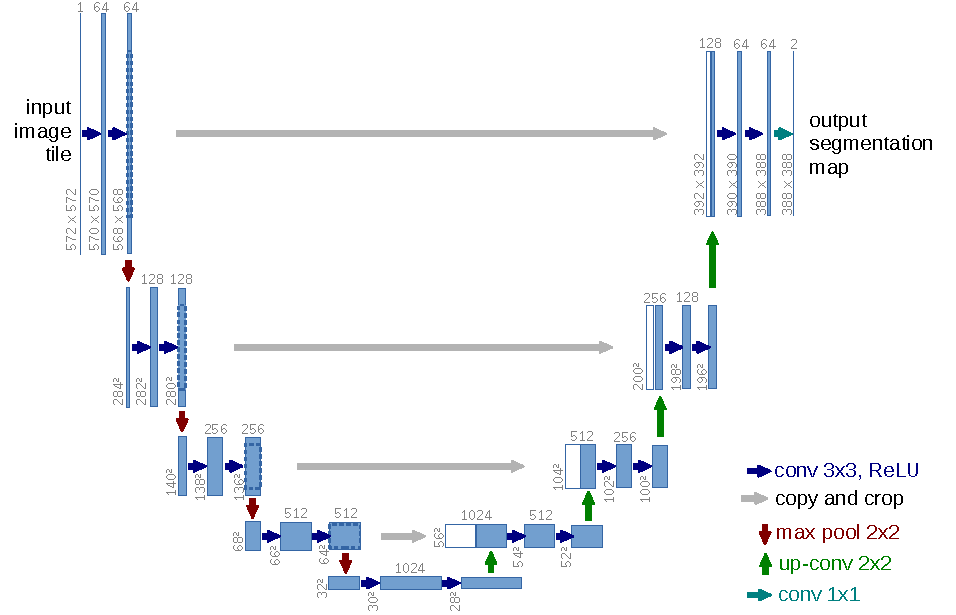
\includegraphics[width=0.65\textwidth]{u-net-illustration-correct-scale2.pdf}
    \caption{UNet architecture}
    \label{unet}
\end{figure}

In practice, these skip connections give the model a significant improvement in image segmentation, where precise localisation is critical and getting both high-resolution and low-resolution images in each layer can help it identify each part better.

The best hyperparameters for this model and the following one were found in a parameter sweep in \cref{param_sweep}.

\subsection{Enhanced Model 2: Swin transformer + JNet \tpdf{\phantom{xx}\small\texttt{models/Swin2Base.py}}}

\begin{figure}
	\centering
	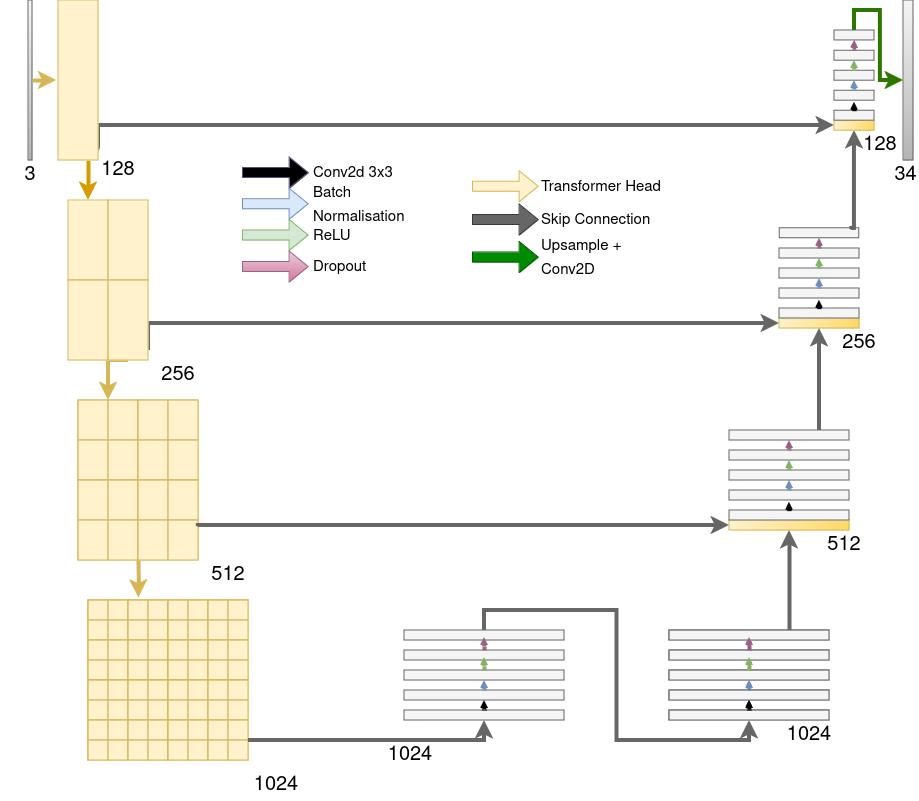
\includegraphics[height=.4\textheight]{Swin2_JNet}
	\caption{Rough outline of Swin2-JNet architecture in use for the Enhanced Model 2. The encoder is a Swin2 tranformer with pre-trained weights; the decoder is a series of upscaling convolutions using the results from the previous step and skip connections from the encoder.}
	\label{swin2}
\end{figure}

Vision Transformers were introduced by the Google Brain team in 2020\cite{vision_transformers}.
To train this model an image is split into $16 \times 16$ patches, each of which is flattened and sent to an attention head.
Each attention head makes its own image segmentation prediction, and all the predictions are finally patched together.

Vision transformers have had good results in many image analysis tasks\cite{vision_transformers_a_survey}.
However, many tests in our codebase of Cityscapes didn't produce results on models using them, so an alternative was needed.

Instead, we use the attention mechanisms in the Swin2 transformers\cite{swin2} to encode the relevant features of the image.
Swin2 uses a more refined architecture mechanism that ViT, such as shifted windows to ensure that the attention heads from one of the patches can be used in the next.

Like most transformers architectures, Swin2 requires a lot of data and time to be trained into something relevant.
Instead of doing this, we leverage transfer learning by using pre-trained weights in the encoder.

The base model of Swin2 encodes the data in 4 attention heads, each one with a smaller image containing more channels of data.
We can leverage this data by getting each of the 4 output feature maps at each step of the way, and adding them as skip connections to up-convolutions in a similar way to UNet in a J-shape.
We call the model ``Swin2-JNet'' for this reason.

Additionally, we noticed that this model tends to overfit earlier than the UNet model.
To prevent this, we added both a \emph{Dropout} and a \emph{Batch Normalisation} layer to each convolutional block; these normalisations tend to improve the performance of the model.

The ideal ratio of dropout was found in a parameter sweep, along with most other parameters, in \cref{param_sweep}.

